\documentclass[../../../include/open-logic-section]{subfiles}

\begin{document}

\olfileid[pt]{sth}{ordinals}{idea}	
\olsection{A Ideia Geral de um Ordinal}

Considere os números naturais, na sua ordem habitual:
\begin{center}
	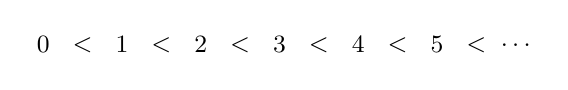
\begin{tikzpicture}
	\foreach \x/\xtext in {0, 1, 2, 3, 4, 5}
	{
		\node (\x a) at (\x, 1) {\small{$\x$}};
		\node (\x a) at (\x.5, 1) {\small{$<$}};
	}
	\node (ldots) at (6, 1) {\small{$\ldots$}};
	\end{tikzpicture}
\end{center}
Chamamos a isto, na gíria, uma $\omega$-sucessão. E, de fato, esta
ordenação geral espelha-se na nossa construção inicial dos estágios
da hierarquia de conjuntos. Mas suponha agora que movemos $0$ para o fim desta
sucessão, de modo que fica depois de todos os outros números:
\begin{center}
	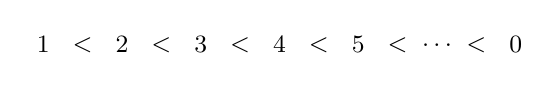
\begin{tikzpicture}
	\foreach \x/\xtext in {1, 2, 3, 4, 5}
	{
		\node (\x a) at (\x, 1) {\small{$\x$}};
		\node (\x a) at (\x.5, 1) {\small{$<$}};
	}
	\node (ldots) at (6, 1) {\small{$\ldots$}};
	\node (bea) at (6.5, 1) {\small{$<$}};
	\node (noa) at (7, 1) {\small{$0$}};
	\end{tikzpicture}
\end{center}
Temos aqui as mesmas entidades, mas ordenadas de modo fundamentalmente
diferente: a nossa primeira ordenação não tinha último elemento; a nova
tem. De fato, a nova ordenação consiste numa
$\omega$-sucessão de entidades ($1, 2, 3, 4, 5, \ldots$), seguida de
outra entidade. Será uma sucessão do tipo $\omega+1$.

Podemos gerar ainda mais tipos de ordenação, usando apenas estas
entidades. Por exemplo, considere todos os números pares (na sua ordem natural)
seguidos de todos os ímpares (na sua ordem natural):
\begin{center}
	\begin{tikzpicture}
	\node(a1) at (1,1) {\small{$0$}};
	\node(a2) at (1.5,1) {\small{$<$}};
	\node(a3) at (2,1) {\small{$2$}};
	\node(a4) at (2.5,1) {\small{$<$}};
	\node(a5) at (3,1) {\small{$4$}};
	\node(a6) at (3.5,1) {\small{$<$}};
	\node(dots) at (4,1) {\small{$\ldots$}};
	\node(aaoe) at (4.5,1) {\small{$<$}};
	\node(b1) at (5,1) {\small{$1$}};
	\node(b2) at (5.5,1) {\small{$<$}};
	\node(b3) at (6,1) {\small{$3$}};
	\node(b4) at (6.5,1) {\small{$<$}};
	\node(b5) at (7,1) {\small{$\ldots$}};
	\end{tikzpicture}
\end{center}
Isto é uma $\omega$-sucessão seguida de outra $\omega$-sucessão; uma
sucessão do tipo $\omega+\omega$. 

Pois bem, podemos continuar. Mas o que gostaríamos é de ter uma forma geral de
entender esta linguagem sobre \emph{ordenações}. 

\end{document}
